% !TeX root = RJwrapper.tex
\title{\pkg{fasano.franceschini.test}: An Implementation of a Multivariate KS Test in R}
\author{by Connor Puritz, Elan Ness-Cohn, Rosemary Braun}

\maketitle
\abstract{%
The Kolmogorov--Smirnov (KS) test is a nonparametric statistical test used to test for differences between univariate probability distributions. The versatility of the KS test has made it a cornerstone of statistical analysis across many scientific disciplines. However, the test proposed by Kolmogorov and Smirnov does not easily extend to multivariate distributions. Here we present the \CRANpkg{fasano.franceschini.test} package, an R implementation of a multivariate two-sample KS test described by \citet{ff1987}. The \pkg{fasano.franceschini.test} package provides a test that is computationally efficient, applicable to data of any dimension and type (continuous, discrete, or mixed), and that performs competitively with similar R packages.
}
 
%%%%%%%%%%%%%%%%%%%%%%%%%%%%%%%%%%%%%%%%%%%%%%%%%%%%%%%%%%%%

\section{Introduction}
\label{introduction}
The Kolmogorov--Smirnov (KS) test is a nonparametric, univariate statistical test designed to assess whether a sample of data is consistent with a given probability distribution (or, in the two-sample case, whether the two samples came from the same underlying distribution). First described by Kolmogorov and Smirnov in a series of papers \citep{Kolmogorov1933, Kolmogorov1933a, Smirnov1936, Smirnov1937, Smirnov1939, Smirnov1944, Smirnov1948}, the KS test is a popular goodness-of-fit test that has found use across a wide variety of scientific disciplines, including neuroscience \citep{atasoy_2017}, climatology \citep{chiang_2018}, robotics \citep{hahne_2018}, epidemiology \citep{wong_2020}, and cell biology \citep{kaczanowska_2021}.

Due to its popularity, several multivariate extensions of the KS test have been described in literature. \citet{justel_1997} proposed a multivariate test based on Rosenblatt's transformation, which reduces to the KS test in the univariate case. While the test statistic is distribution-free, it is difficult to compute in more than two dimensions, and an approximate test with reduced power must be used instead. Furthermore, the test is only applicable in the one-sample case. \citet{heuchenne_2022} proposed to use the Hilbert space-filling curve to define an ordering in $\mathbb{R}^{2}$. The preimage of both samples is computed under the space-filling curve map, and the two-sample KS test is performed on the preimages. While it is theoretically possible to extend this approach to higher dimensions, the authors note that this would be computationally challenging and leave it as an open problem. \citet{naaman_2021} derived a multivariate extension of the DKW inequality and used it to provide estimates of the tail properties of the asymptotic distribution of the KS test statistic in multiple dimensions. While an important theoretical result, it is of limited practical use absent a method for computing exact $p$-values.

\citet{peacock_1983} proposed a test which addresses the fact that there are multiple ways to order points in higher dimensions, and thus multiple ways of defining a cumulative distribution function. In one dimension, probability density can be integrated from left to right, resulting in the canonical CDF $P(X<x)$; or from right to left, resulting in the survival function $P(X>x)$. However, since $P(X<x)=1-P(X>x)$ (for continuous random variables), the KS test statistic is independent of this choice. In two dimensions, there are four ways of ordering points, and thus four possible cumulative distribution functions: $P(X<x,Y<y)$, $P(X>x,Y<y)$, $P(X<x,Y>y)$, and $P(X>x,Y>y)$. Since any three of these are independent of one another, the KS test statistic will not be independent of which ordering is chosen. To address this, \citet{peacock_1983} proposed to compute a KS statistic using each possible cumulative distribution function, and to take the test statistic to be the maximum of those.

\citet{peacock_1983} suggested that for a sample $(X_{1},Y_{1}),\dots,(X_{n},Y_{n})$, each of the four KS statistics should be maximized over the set of all coordinate-wise combinations $\{(X_{i},Y_{j}):1\leq i,j\leq n\}$. The complexity of computing Peacock's test statistic thus scales cubically with sample size, which is expensive and can become intractable for large sample sizes. \citet{ff1987} proposed a simple change to Peacock's test: instead of maximizing each KS statistic over all coordinate-wise combinations of points in the sample, the statistics should be maximized over just the points in the sample itself. This slight change greatly reduces the computational complexity of the test while maintaining a similar power across a variety of alternatives \citep{ff1987,lopes_2007}. \citet{ff1987} proposed both a one-sample and two-sample version of their test, although we focus on the two-sample test here.

In this article we present the \pkg{fasano.franceschini.test} package, an R implementation of the two-sample Fasano--Franceschini test. Our implementation can be applied to continuous, discrete, or mixed datasets of any size and of any dimension. We first introduce the test by detailing how the test statistic is computed, how it can be computed efficiently, and how $p$-values can be computed. We then describe the package structure and provide several basic examples illustrating its usage. We conclude by comparing the package to three other CRAN packages implementing multivariate two-sample goodness-of-fit tests.

%%%%%%%%%%%%%%%%%%%%%%%%%%%%%%%%%%%%%%%%%%%%%%%%%%%%%%%%%%%%

\section{Fasano--Franceschini test}
\subsection{Two-sample test statistic}
Let $\mathbf{X}=(\mathbf{X}_{1},\dots,\mathbf{X}_{n_{1}})$ and $\mathbf{Y}=(\mathbf{Y}_{1},\dots,\mathbf{Y}_{n_{2}})$ be samples of i.i.d.\ $d$-dimensional random vectors drawn from unknown distributions $F_{1}$ and $F_{2}$, respectively. The two-sample Fasano--Franceschini test evaluates the null hypothesis
\begin{equation*}
H_{0}:F_{1}=F_{2}
\end{equation*}
against the alternative
\begin{equation*}
H_{1}:F_{1}\neq F_{2}.
\end{equation*}
In their original paper, \citet{ff1987} only considered two- and three-dimensional random vectors, although their test naturally extends to arbitrary dimensions as follows.

For $\mathbf{x}\in\mathbb{R}^{d}$, we define the $i$th open orthant with origin $\mathbf{x}$ as
\begin{equation*}
\mathcal{O}_{i}(\mathbf{x})=\left\{\mathbf{y}\in\mathbb{R}^{d}\,\rvert\,\mathbf{e}_{ij}(\mathbf{y}_{j}-\mathbf{x}_{j})>0,\;j=1,\dots,d\right\}
\end{equation*}
where $\mathbf{e}_{i}\in\{-1,1\}^{d}$ is a length $d$ combination of $\pm 1$. For example, in two dimensions, the four combinations $\mathbf{e}_{1}=(1,1)$, $\mathbf{e}_{2}=(-1,1)$, $\mathbf{e}_{3}=(-1,-1)$, and $\mathbf{e}_{4}=(1,-1)$ correspond to quadrants one through four in the plane, respectively. In general there are $2^{d}$ such combinations, corresponding to the $2^{d}$ orthants that divide $\mathbb{R}^{d}$. Using the indicator function
\begin{equation*}
I_{j}(\mathbf{x}\,\rvert\,\mathbf{y})=
\begin{cases}
1,\hfill&\mathbf{x}\in\mathcal{O}_{j}(\mathbf{y})\\
0,\hfill&\mathbf{x}\notin\mathcal{O}_{j}(\mathbf{y})
\end{cases}
\end{equation*}
we define
\begin{equation}
\label{eq:diff}
D(\mathbf{p}\,\rvert\,\mathbf{X},\mathbf{Y})=\max_{1\leq j\leq 2^{d}}\left|\frac{1}{n_{1}}\sum_{k=1}^{n_{1}}I_{j}\left(\mathbf{X}_{k}\,\rvert\,\mathbf{p}\right)-\frac{1}{n_{2}}\sum_{k=1}^{n_{2}}I_{j}\left(\mathbf{Y}_{k}\,\rvert\,\mathbf{p}\right)\right|.
\end{equation}
This is similar to the distance used in the two-sample KS test, but takes into account all possible ways of ordering points in $\mathbb{R}^{d}$. Note that this function does not depend on the enumeration of the orthants. Maximizing $D$ over each sample separately leads to the difference statistics
\begin{equation*}
D_{1}(\mathbf{X},\mathbf{Y})=\max_{1\leq i\leq n_{1}}D(\mathbf{X}_{i}\,\rvert\,\mathbf{X},\mathbf{Y})
\end{equation*}
and
\begin{equation*}
D_{2}(\mathbf{X},\mathbf{Y})=\max_{1\leq i\leq n_{2}}D(\mathbf{Y}_{i}\,\rvert\,\mathbf{X},\mathbf{Y}).
\end{equation*}
The two-sample Fasano--Franceschini test statistic, as originally defined by \citet{ff1987}, is the average of the difference statistics scaled by the sample sizes:
\begin{equation}
\label{eq:ff_stat}
\mathcal{D}_{0}(\mathbf{X},\mathbf{Y})=\sqrt{\frac{n_{1}n_{2}}{n_{1}+n_{2}}}\left(\frac{D_{1}(\mathbf{X},\mathbf{Y})+D_{2}(\mathbf{X},\mathbf{Y})}{2}\right).
\end{equation}
This test statistic is discrete, but in general is not integer-valued. Note that
\begin{equation*}
n_{1}n_{2}D(\mathbf{p}\,\rvert\,\mathbf{X},\mathbf{Y})=\max_{1\leq j\leq 2^{d}}\left|n_{2}\sum_{k=1}^{n_{1}}I_{j}\left(\mathbf{X}_{k}\,\rvert\,\mathbf{p}\right)-n_{1}\sum_{k=1}^{n_{2}}I_{j}\left(\mathbf{Y}_{k}\,\rvert\,\mathbf{p}\right)\right|\in\mathbb{Z},
\end{equation*}
and thus
\begin{equation*}
n_{1}n_{2}D_{i}(\mathbf{X},\mathbf{Y})\in\mathbb{Z},\;i\in\{1,2\}.
\end{equation*}
Let
\begin{equation*}
C_{n_{1},n_{2}}=2\sqrt{n_{1}n_{2}(n_{1}+n_{2})}.
\end{equation*}
Then
\begin{align*}
C_{n_{1},n_{2}}\mathcal{D}_{0}(\mathbf{X},\mathbf{Y})&=2\sqrt{n_{1}n_{2}(n_{1}+n_{2})}\sqrt{\frac{n_{1}n_{2}}{n_{1}+n_{2}}}\left(\frac{D_{1}(\mathbf{X},\mathbf{Y})+D_{2}(\mathbf{X},\mathbf{Y})}{2}\right)\\&=n_{1}n_{2}(D_{1}(\mathbf{X},\mathbf{Y})+D_{2}(\mathbf{X},\mathbf{Y}))\in\mathbb{Z}.
\end{align*}
To avoid comparing floating point numbers, it is preferable for the test statistic to be integer-valued, and thus we use
\begin{equation}
\label{eq:test_stat}
\mathcal{D}(\mathbf{X},\mathbf{Y})=C_{n_{1},n_{2}}\mathcal{D}_{0}(\mathbf{X},\mathbf{Y})
\end{equation}
as our test statistic. As will be shown, the $p$-value of the test is independent of scalar rescaling of the test statistic.

\begin{figure}[htbp]
\centering
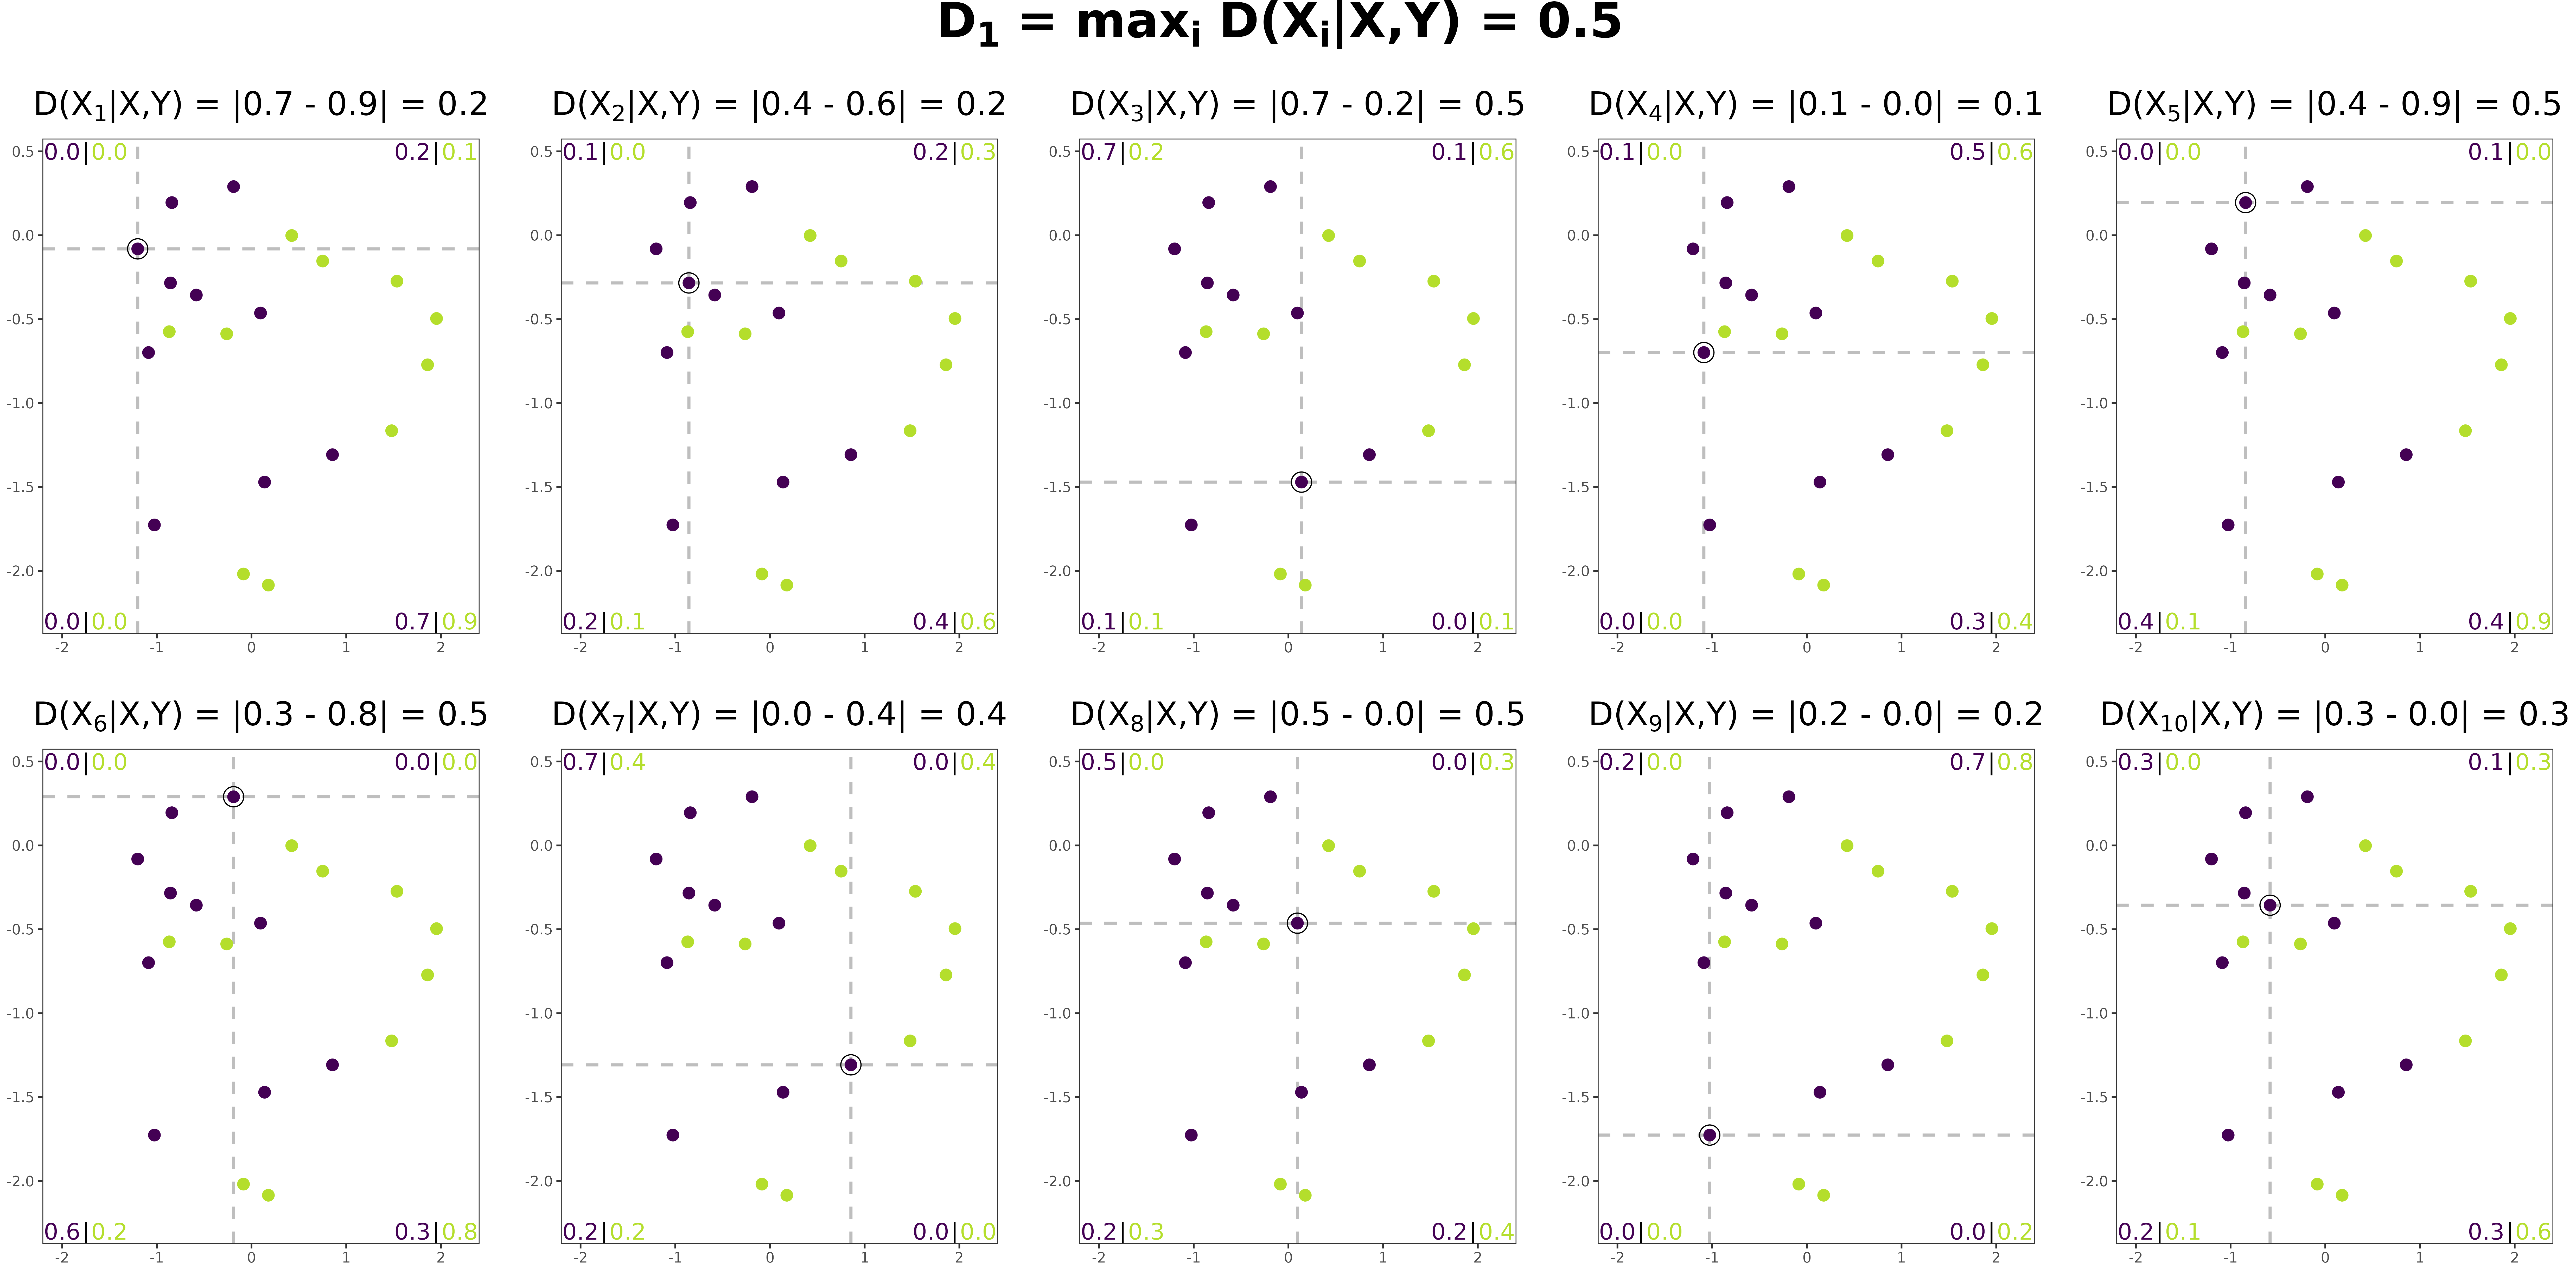
\includegraphics[scale=0.248]{figures/fig1.png}
\caption{Illustration of the computation of the difference statistic $D_{1}$ in two dimensions. Each point in the first sample is used to divide the plane into four quadrants, and both samples are cumulated in each of the four quadrants. The fraction of each sample in each quadrant is shown in the corresponding plot corner, and the maximum difference over all four quadrants is shown above each plot. $D_{1}$ is taken as the maximum of these differences. To compute the test statistic, we would next compute $D_{2}$ by repeating the same procedure, but using points in the second sample to divide the plane instead.}
\label{figure:example_stat}
\end{figure}

%%%%%%%%%%%%%%%%%%%%%%%%%%%%%%%%%%%%%%%%%%%%%%%%%%%%%%%%%%%%

\subsection{Computational complexity}
The bulk of the time required to compute the test statistic in (\ref{eq:test_stat}) is spent evaluating sums of the form
\begin{equation*}
\sum_{\mathbf{x}\in S}I_{j}\left(\mathbf{x}\,\rvert\,\mathbf{y}\right),
\end{equation*}
which count the number of points in a set $S$ that lie in a given $d$-dimensional region. The simplest approach to computing such sums is brute force, where every point $\mathbf{x}\in S$ is checked independently. The orthant a point lies in can be determined using $d$ binary checks, resulting in a time complexity of $O(N^{2})$, where $N=\max(n_{1},n_{2})$, to evaluate (\ref{eq:test_stat}) for fixed $d$.

Alternatively, we can consider each sum as a single query rather than a sequence of independent ones. Specifically, both sums in (\ref{eq:diff}) are orthogonal range counting queries, which ask how many points in a set $S\subset\mathbb{R}^{d}$ lie in an axis-aligned box $(x_{1},x_{1}')\times\dots \times(x_{d},x_{d}')$. Range counting is an important problem in the field of computational geometry, and as such a variety of data structures have been described to provide efficient solutions \citep{geometry_2008}. One solution, first introduced by \citet{bentley_decomposable_1979}, is a multi-layer binary search tree termed a range tree. Other slightly more efficient data structures have been proposed for range counting, but range trees are well suited for our purposes, particularly because their construction scales easily to arbitrary dimensions \citep{bentley_decomposable_1979, geometry_2008}.

A range tree can be constructed on a set of $n$ points in $d$-dimensional space using $O(n\log^{d-1}n)$ space in $O(n\log^{d-1}n)$ time. The number of points that lie in an axis-aligned box can be reported in $O(\log^{d}n)$ time, and this time can be further reduced to $O(\log^{d-1}n)$ when $d>1$ using fractional cascading \citep{geometry_2008}. To compute (\ref{eq:test_stat}), we construct one range tree for each of the two samples, and then query each tree $2^{d}$ times. Thus the total time complexity to compute the test statistic using range trees for fixed $d$ is $O(N\log^{d-1}N)$, where $N=\max(n_{1},n_{2})$.

\begin{figure}[htbp]
\centering

\includegraphics[scale=0.50]{figures/fig2.png}
\caption{Time to compute the Fasano--Franceschini test statistic as a function of sample size, comparing the brute force and range tree methods for data of dimensions two through five. Points represent the mean time of $200$ evaluations. Samples are taken to be of the same size and are drawn from multivariate standard normal distributions.}
\label{figure:stat_time}
\end{figure}

As the range tree method has a better asymptotic time complexity, we expect it to outperform the brute force method for larger sample sizes. However, for smaller sample sizes, the cost of building the range trees can outweigh the benefit gained by more efficient querying. As exact computation times can vary depending on the geometry of the samples, it is not possible to determine in general when one method will outperform the other. Despite this, we sought to establish rough benchmarks. Drawing equal sized samples from multivariate standard normal distributions, we sought to determine the sample size $N^{*}$ at which the range tree method becomes more efficient than the brute force method (Figure~\ref{figure:stat_time}). For $d=2$, $N^{*}\approx 25$; for $d=3$, $N^{*}\approx 200$; for $d=4,5$, and presumably all higher dimensions, $N^{*}>4000$. Based on these benchmarking results, our package automatically selects which of the two methods is likely faster based on the dimension and samples sizes of the supplied data. If users are interested in performing more precise benchmarking for their specific dataset, the argument \code{nPermute} can be set equal to $0$, which bypasses the permutation test and only computes the test statistic.

%%%%%%%%%%%%%%%%%%%%%%%%%%%%%%%%%%%%%%%%%%%%%%%%%%%%%%%%%%%%

\subsection{Significance testing}
To the best of our knowledge, no results have been published concerning the distribution of the Fasano--Franceschini test statistic. Any analysis would likely be complicated by the fact that, unlike the KS test statistic, the Fasano--Franceschini test statistic is not distribution free \citep{ff1987}. In their original paper, \citet{ff1987} did not attempt any analytical analysis and instead performed simulations to estimate critical values of their test statistic for various two- and three-dimensional distributions. By fitting a curve to their results, \citet{press2007} proposed an explicit formula for $p$-values in the two-dimensional case. However, this formula is only approximate, and its accuracy degrades as sample sizes decrease or the true $p$-value becomes large (greater than $0.2$). While this would still allow a simple rejection decision at any common significance level, it is sometimes useful to quantify large $p$-values more exactly (such as if one was to do a cross-study concordance analysis comparing $p$-values between studies as in \citealt{ness-cohn_2020}). Effort could be made to improve this approximation, however it is still only valid in two dimensions, and thus an alternative method would be needed in higher dimensions.

To ensure the broadest applicability of the test, we assess significance using a permutation test. Let $\mathbf{Z}=(\mathbf{Z}_{1},\dots,\mathbf{Z}_{N})$ be defined by
\begin{equation*}
\mathbf{Z}_{i}=\begin{cases}
\mathbf{X}_{i},&1\leq i\leq n_{1}\\
\mathbf{Y}_{i-n_{1}},&n_{1}+1\leq i\leq N
\end{cases}
\end{equation*}
where $N=n_{1}+n_{2}$. The test statistic in (\ref{eq:test_stat}) can then be written as
\begin{equation*}
\mathcal{D}(\mathbf{Z})=\mathcal{D}(\mathbf{X},\mathbf{Y}).
\end{equation*}
Denote the symmetric group on $\{1,\dots,n\}\subset\mathbb{N}$ by $S_{n}$. For $\mathbf{x}=(\mathbf{x}_{1},\dots,\mathbf{x}_{n})$ and $\sigma\in S_{n}$, define
\begin{equation*}
\mathbf{x}_{\sigma}=(\mathbf{x}_{\sigma(1)},\dots,\mathbf{x}_{\sigma(n)}).
\end{equation*}
Under the null hypothesis, $\mathbf{X}$ and $\mathbf{Y}$ were drawn from the same distribution, and thus the elements of $\mathbf{Z}$ are exchangeable. We can therefore compute the permutation test p-value
\begin{equation}
p=\frac{\sum_{\sigma\in S_{N}}I(\mathcal{D}(\mathbf{Z}_{\sigma})\geq\mathcal{D}(\mathbf{Z}))}{N!}
\end{equation}
where $I$ denotes the indicator function \citep{hemerik2018,ramdas2022permutation}. As it is generally infeasible to iterate over all $N!$ permutations, we can instead consider for $M\in\mathbb{N}$
\begin{equation}
p_{M}=\frac{1+\sum_{m=1}^{M}I(\mathcal{D}(\mathbf{Z}_{\sigma_{m}})\geq\mathcal{D}(\mathbf{Z}))}{1+M}
\end{equation}
where $\sigma_{1},\dots,\sigma_{M}$ are independent permutations drawn uniformly from $S_{N}$. This $p$-value is valid, as under the null hypothesis
\begin{equation*}
\mathbb{P}(p_{m}\leq\alpha)\leq\alpha \ \forall\alpha\in[0,1].
\end{equation*}
Moreover, $p_{M}\to p$ almost surely. These results hold for any sampling distributions (continuous, discrete, or mixed) and any valid test statistic \citep{hemerik2018, ramdas2022permutation}.

\begin{figure}[htbp]
\centering
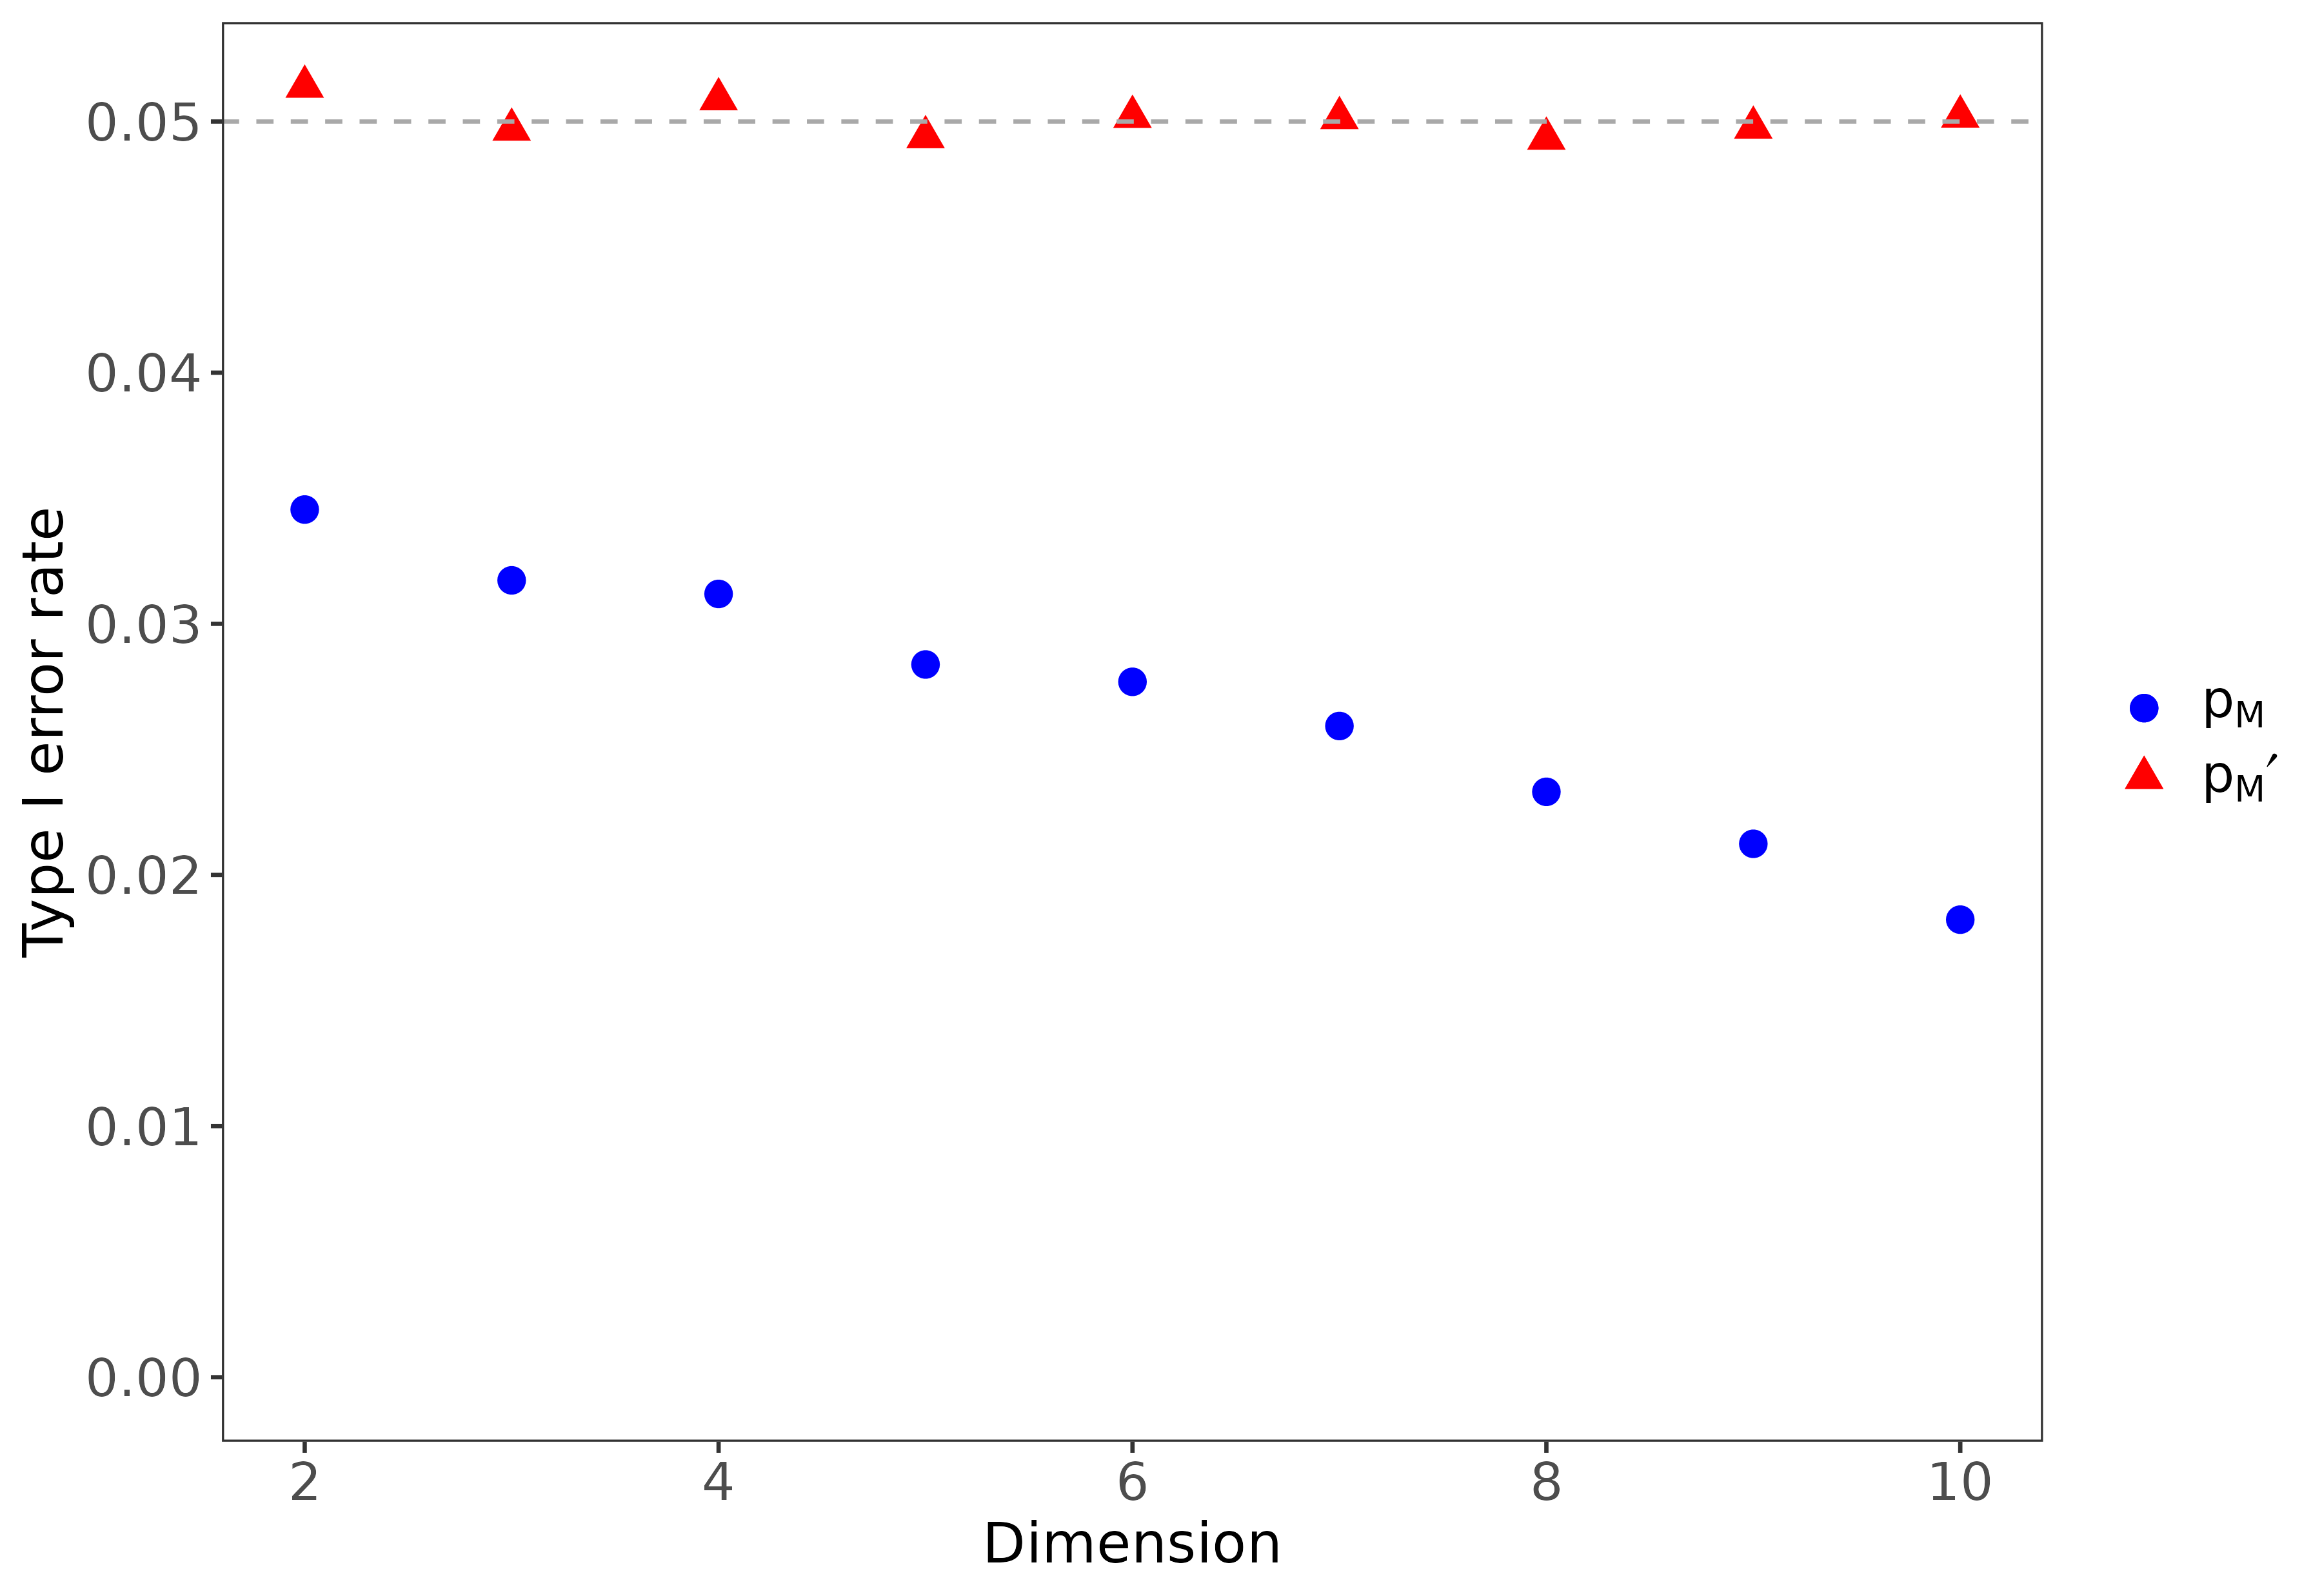
\includegraphics[scale=0.4]{figures/fig3.png}
\caption{Type I error rate of the test using $p_{M}$ and $p_{M}'$ as dimension increases. Samples are both of size $10$ and are drawn from standard multivariate normal distributions of the specified dimension. The number of permutations used is $100$, and the error rate is estimated using $10^{5}$ replications.}
\label{figure:pvalues}
\end{figure}

Under certain conditions (see Proposition 2 of \citealt{hemerik2018}), the permutation test using the $p$-value $p_{M}$ is exact, which is to say that under the null hypothesis
\begin{equation*}
\mathbb{P}(p_{m}\leq\alpha)=\alpha \ \forall\alpha\in[0,1].
\end{equation*}
However, when there is a nonzero probability of ties in the test statistic, this test can be quite conservative \citep{hemerik2018}. In such cases, the test can be made exact by instead using
\begin{equation}
p_{M}'=\frac{\sum_{m=1}^{M}I(\mathcal{D}(\mathbf{Z}_{\sigma_{m}})>\mathcal{D}(\mathbf{Z}))}{1+M}+U\frac{1+\sum_{m=1}^{M}I(\mathcal{D}(\mathbf{Z}_{\sigma_{m}})=\mathcal{D}(\mathbf{Z}))}{1+M}\,,
\end{equation}
where $U\sim\mathrm{Unif}(0,1)$ \citep{hoeffding1952,hemerik2018}. The fact that $p_{M}'$ is randomized is not inherently problematic, since it is already randomized due to the selection of random permutations \citep{hemerik2018}.

As the test statistic in (\ref{eq:test_stat}) is discrete, ties are possible, and thus the test using $p_{M}$ is generally conservative.  In high dimensions, ties can become quite prevalent, leading the type I error rate to decrease dramatically (Figure~\ref{figure:pvalues}). We thus use $p_{M}'$ as our $p$-value instead of $p_{M}$. As a final remark, we note that if the test statistic is scaled by a constant scalar, $p_{M}'$ remains unchanged since both indicator functions are invariant under scalar rescaling of $\mathcal{D}$. Therefore, the outcome of the test does not depend on our choice to use the integer-valued test statistic $\mathcal{D}$ in (\ref{eq:test_stat}) over Fasano and Franceschini's original test statistic $\mathcal{D}_{0}$ in (\ref{eq:ff_stat}).

%%%%%%%%%%%%%%%%%%%%%%%%%%%%%%%%%%%%%%%%%%%%%%%%%%%%%%%%%%%%

\section{Package overview}
The \pkg{fasano.franceschini.test} package is written primarily in C++, and interfaces with R using \CRANpkg{Rcpp} \citep{rcpp}. The C++ range tree class \citep{rtreeGithub} was based on the description in \citet{geometry_2008}, including an implementation of fractional cascading. The permutation test is parallelized using \CRANpkg{RcppParallel} \citep{rcppparallel}. The package consists of one function, \code{fasano.franceschini.test}, for performing the two-sample Fasano--Franceschini test. The arguments of this function are described below.
\begin{itemize}
\item \code{S1} and \code{S2}: the two samples to compare. Both should be either numeric \code{matrix} or \code{data.frame} objects with the same number of columns.
\item \code{nPermute}: the number of permutations to use for performing the permutation test. The default is $100$. If set equal to $0$, the permutation test is bypassed and only the test statistic is computed.
\item \code{threads}: the number of threads to use when performing the permutation test. The default is one thread. This parameter can also be set to \code{"auto"}, which uses the value returned by \code{RcppParallel::defaultNumThreads()}.
\item \code{seed}: an optional seed for the pseudorandom number generator (PRNG) used during the permutation test.
\item \code{verbose}: whether to display a progress bar while performing the permutation test. The default is \code{TRUE}. This functionality is only available when \code{threads = 1}.
\item \code{method}: an optional \code{character} indicating which method to use to compute the test statistic. The two methods are \code{'r'} (range tree) and \code{'b'} (brute force). Both methods return the same results but may vary in computation speed. If this argument is not passed, the sample sizes and dimension of the data are used to infer which method is likely faster.
\end{itemize}
The output is an object of the class \code{htest}, and consists of the following components:
\begin{itemize}
\item \code{statistic}: the value of the test statistic.
\item \code{p.value}: the permutation test p-value.
\item \code{method}: the name of the test (i.e. \code{'Fasano-Franceschini Test'}).
\item \code{data.name}: the names of the original data objects.
\end{itemize}

%%%%%%%%%%%%%%%%%%%%%%%%%%%%%%%%%%%%%%%%%%%%%%%%%%%%%%%%%%%%

\section{Examples}
Here we demonstrate the basic usage and features of the \pkg{fasano.franceschini.test} package. We begin by loading the necessary libraries and setting a seed for reproducibility.
\begin{example}
> library(fasano.franceschini.test)
> library(MASS)
> set.seed(0)
\end{example}
Note that to produce reproducible results, we need to set two seeds: the \texttt{set.seed} function sets the seed in R, ensuring we draw reproducible samples; and the seed passed as an argument to the \texttt{fasano.franceschini.test} function sets the seed for the C++ PRNG, ensuring we compute reproducible $p$-values.

As a first example, we draw two samples from the bivariate standard normal distribution. The Fasano--Franceschini test fails to reject the null hypothesis --- that the samples were drawn from the same distribution --- at an $\alpha=0.05$ significance level.

\begin{example}
> S1 <- mvrnorm(n = 50, mu = c(0, 0), Sigma = diag(2))
> S2 <- mvrnorm(n = 75, mu = c(0, 0), Sigma = diag(2))
> fasano.franceschini.test(S1, S2, seed = 1, verbose = FALSE)

	Fasano-Franceschini Test

data:  S1 and S2
D = 1425, p-value = 0.4653
\end{example}

We next draw two samples from bivariate normal distributions with identical covariance matrices but different locations. The test rejects the null hypothesis at an $\alpha=0.05$ significance level.

\begin{example}
> S3 <- mvrnorm(n = 40, mu = c(0, 0), Sigma = diag(2))
> S4 <- mvrnorm(n = 42, mu = c(1, 1), Sigma = diag(2))
> fasano.franceschini.test(S3, S4, seed = 2, verbose = FALSE)

	Fasano-Franceschini Test

data:  S3 and S4
D = 1932, p-value = 0.001832
\end{example}

The test can take a while to run when the sample sizes or the dimension of the data are large, in which case it is useful to use multiple threads to speed up computation.

\begin{example}
> S5 <- mvrnorm(n = 1000, mu = c(1, 3, 5), Sigma = diag(3) + 1)
> S6 <- mvrnorm(n = 600, mu = c(1, 3, 5), Sigma = diag(3))
> fasano.franceschini.test(S5, S6, seed = 3, threads = 4)

	Fasano-Franceschini Test

data:  S5 and S6
D = 263800, p-value = 0.0007002
\end{example}

Note that the number of threads used does not affect the results. In particular, as long as the same seed is used, the same $p$-value is returned for any number of threads.
\begin{example}
> fasano.franceschini.test(S5, S6, seed = 3, threads = 1)

	Fasano-Franceschini Test

data:  S5 and S6
D = 263800, p-value = 0.0007002
\end{example}

%%%%%%%%%%%%%%%%%%%%%%%%%%%%%%%%%%%%%%%%%%%%%%%%%%%%%%%%%%%%

\section{Comparison with other R packages}
In this section, we compare the \pkg{fasano.franceschini.test} package with three other CRAN packages that perform multivariate two-sample goodness-of-fit tests.

\subsection{Peacock.test}
The \CRANpkg{Peacock.test} package \citep{peacockR} provides functions to compute Peacock's test statistic \citep{peacock_1983} in two and three dimensions. As no function is provided to compute $p$-values, we cannot directly compare the performance of this package with the \pkg{fasano.franceschini.test} package. However, a treatment of the power of both Peacock and Fasano--Franceschini tests can be found in both the primary literature \citep{peacock_1983,ff1987} and in a subsequent benchmarking paper \citep{lopes_2007}, which found that the two tests have similar power across a variety of alternatives.

\subsection{cramer}
The \CRANpkg{cramer} package \citep{cramerR} implements the two-sample test described in \citet{baringhaus_2004}, which the authors refer to as the Cram\'er test. The Cram\'er test statistic is based on the Euclidean inter-point distances between the two samples, and is given by
\begin{equation*}
T_{m,n}=\frac{mn}{m+n}\left(\frac{2}{mn}\sum_{i=1}^{m}\sum_{j=1}^{n}\phi\left(\left\lVert\mathbf{X}_{i}-\mathbf{Y}_{j}\right\rVert_{2}^{2}\right)-\frac{1}{m^{2}}\sum_{i,j=1}^{m}\phi\left(\left\lVert\mathbf{X}_{i}-\mathbf{X}_{j}\right\rVert_{2}^{2}\right)-\frac{1}{n^{2}}\sum_{i,j=1}^{n}\phi\left(\left\lVert\mathbf{Y}_{i}-\mathbf{Y}_{j}\right\rVert_{2}^{2}\right)\right)
\end{equation*}
for samples $\mathbf{X}_{1},\dots,\mathbf{X}_{m}$ and $\mathbf{Y}_{1},\dots,\mathbf{Y}_{n}$. The default kernel function is $\phi(x)=\sqrt{x}/2$, although several other choices are implemented (see the documentation for more details). Several randomization methods are provided to compute $p$-values, including bootstrapping (the default) and a permutation test.

\subsection{diproperm}
The \CRANpkg{diproperm} package \citep{dipropermR} implements the DiProPerm test introduced by \citet{diproperm_original}. A binary linear classifier is first trained to determine a separating hyperplane between the two samples. The data are then projected onto the normal vector to the hyperplane, and the test statistic is taken to be a univariate statistic of the projected data (by default the absolute difference of means). As in the \pkg{fasano.franceschini.test} package, significance is determined using a permutation test.

\subsection{Power comparison}
To compare the \pkg{fasano.franceschini.test} package with the \pkg{cramer} and \pkg{diproperm} packages, we performed power analyses using three classes of alternatives: location alternatives, where the means of the marginals are varied; dispersion alternatives, where the variances of the marginals are varied; and copula alternatives, where the marginals remain fixed but the copula joining them is varied.

\begin{figure}[htbp]
\centering
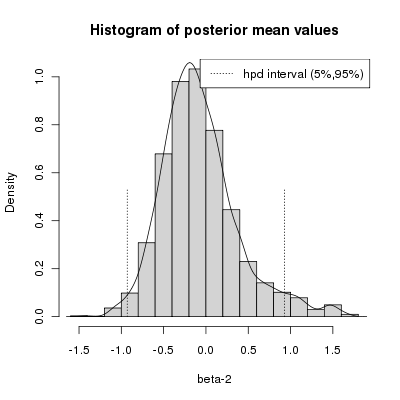
\includegraphics[scale=0.50]{figures/fig4.png}
\caption{Visualization of the distributions used in power analyses. Each plot shows two samples consisting of $10000$ points each. The first sample $S_{1}$ is shown in blue, and the second sample $S_{2}$ is shown in red. (a) $S_{1}\sim N_{2}(\mathbf{0},\mathbf{I}_{2})$ and $S_{2}\sim N_{2}(\mathbf{0.4},\mathbf{I}_{2})$. (b) $S_{1}\sim N_{2}(\mathbf{0},\mathbf{I}_{2})$ and $S_{2}\sim N_{2}(\mathbf{0},\mathbf{I}_{2}+1.5)$. (c) $S_{1}\sim G_{2}(0)$ and $S_{2}\sim G_{2}(0.6)$. (d) $S_{1}\sim C_{2}(1)$ and $S_{2}\sim C_{2}(8)$.}
\label{figure:power_dist}
\end{figure}

For location and dispersion alternatives, we used multivariate normal distributions. We denote the $d$-dimensional normal distribution with mean $\boldsymbol\mu\in\mathbb{R}^{d}$ and covariance matrix $\boldsymbol\Sigma\in\mathbb{R}^{d\times d}$ by $N_{d}(\boldsymbol\mu,\boldsymbol\Sigma)$, and sample from it using the \CRANpkg{MASS} package \citep{mass}. The $d\times d$ identity matrix, which is sometimes used as a covariance matrix, is denoted by $\mathbf{I}_{d}$. For copula alternatives, we consider the Gaussian copula with correlation matrix
\begin{equation*}
[\mathbf{P}(\rho)]_{ij}=\begin{cases}
\rho,&i\neq j\\
1,&i=j
\end{cases}
\end{equation*}
and the Clayton copula with parameter $\theta\in[-1,\infty)\setminus\{0\}$. We denote the $d$-dimensional distribution with standard normal marginals joined by a Gaussian copula with correlation matrix $\mathbf{P}(\rho)$ by $G_{d}(\rho)$. We denote the $d$-dimensional distribution with standard normal marginals joined by a Clayton copula with parameter $\theta$ by $C_{d}(\theta)$. Both distributions are sampled from using the \CRANpkg{copula} package \citep{copulaR}. Examples of distributions in each of these four families are shown in Figure~\ref{figure:power_dist}.

In the following analyses, power was approximated using $1000$ replications, a significance level of $\alpha=0.05$ was used, all samples were of size $40$, and all R functions implementing tests were called using their default arguments. Although we aimed to cover a wide range of distributions in this analysis, absent any theoretical results concerning these three tests, we cannot guarantee that the results here are generalizable to different sampling distributions or sample sizes.

\begin{figure}[htbp]
\centering
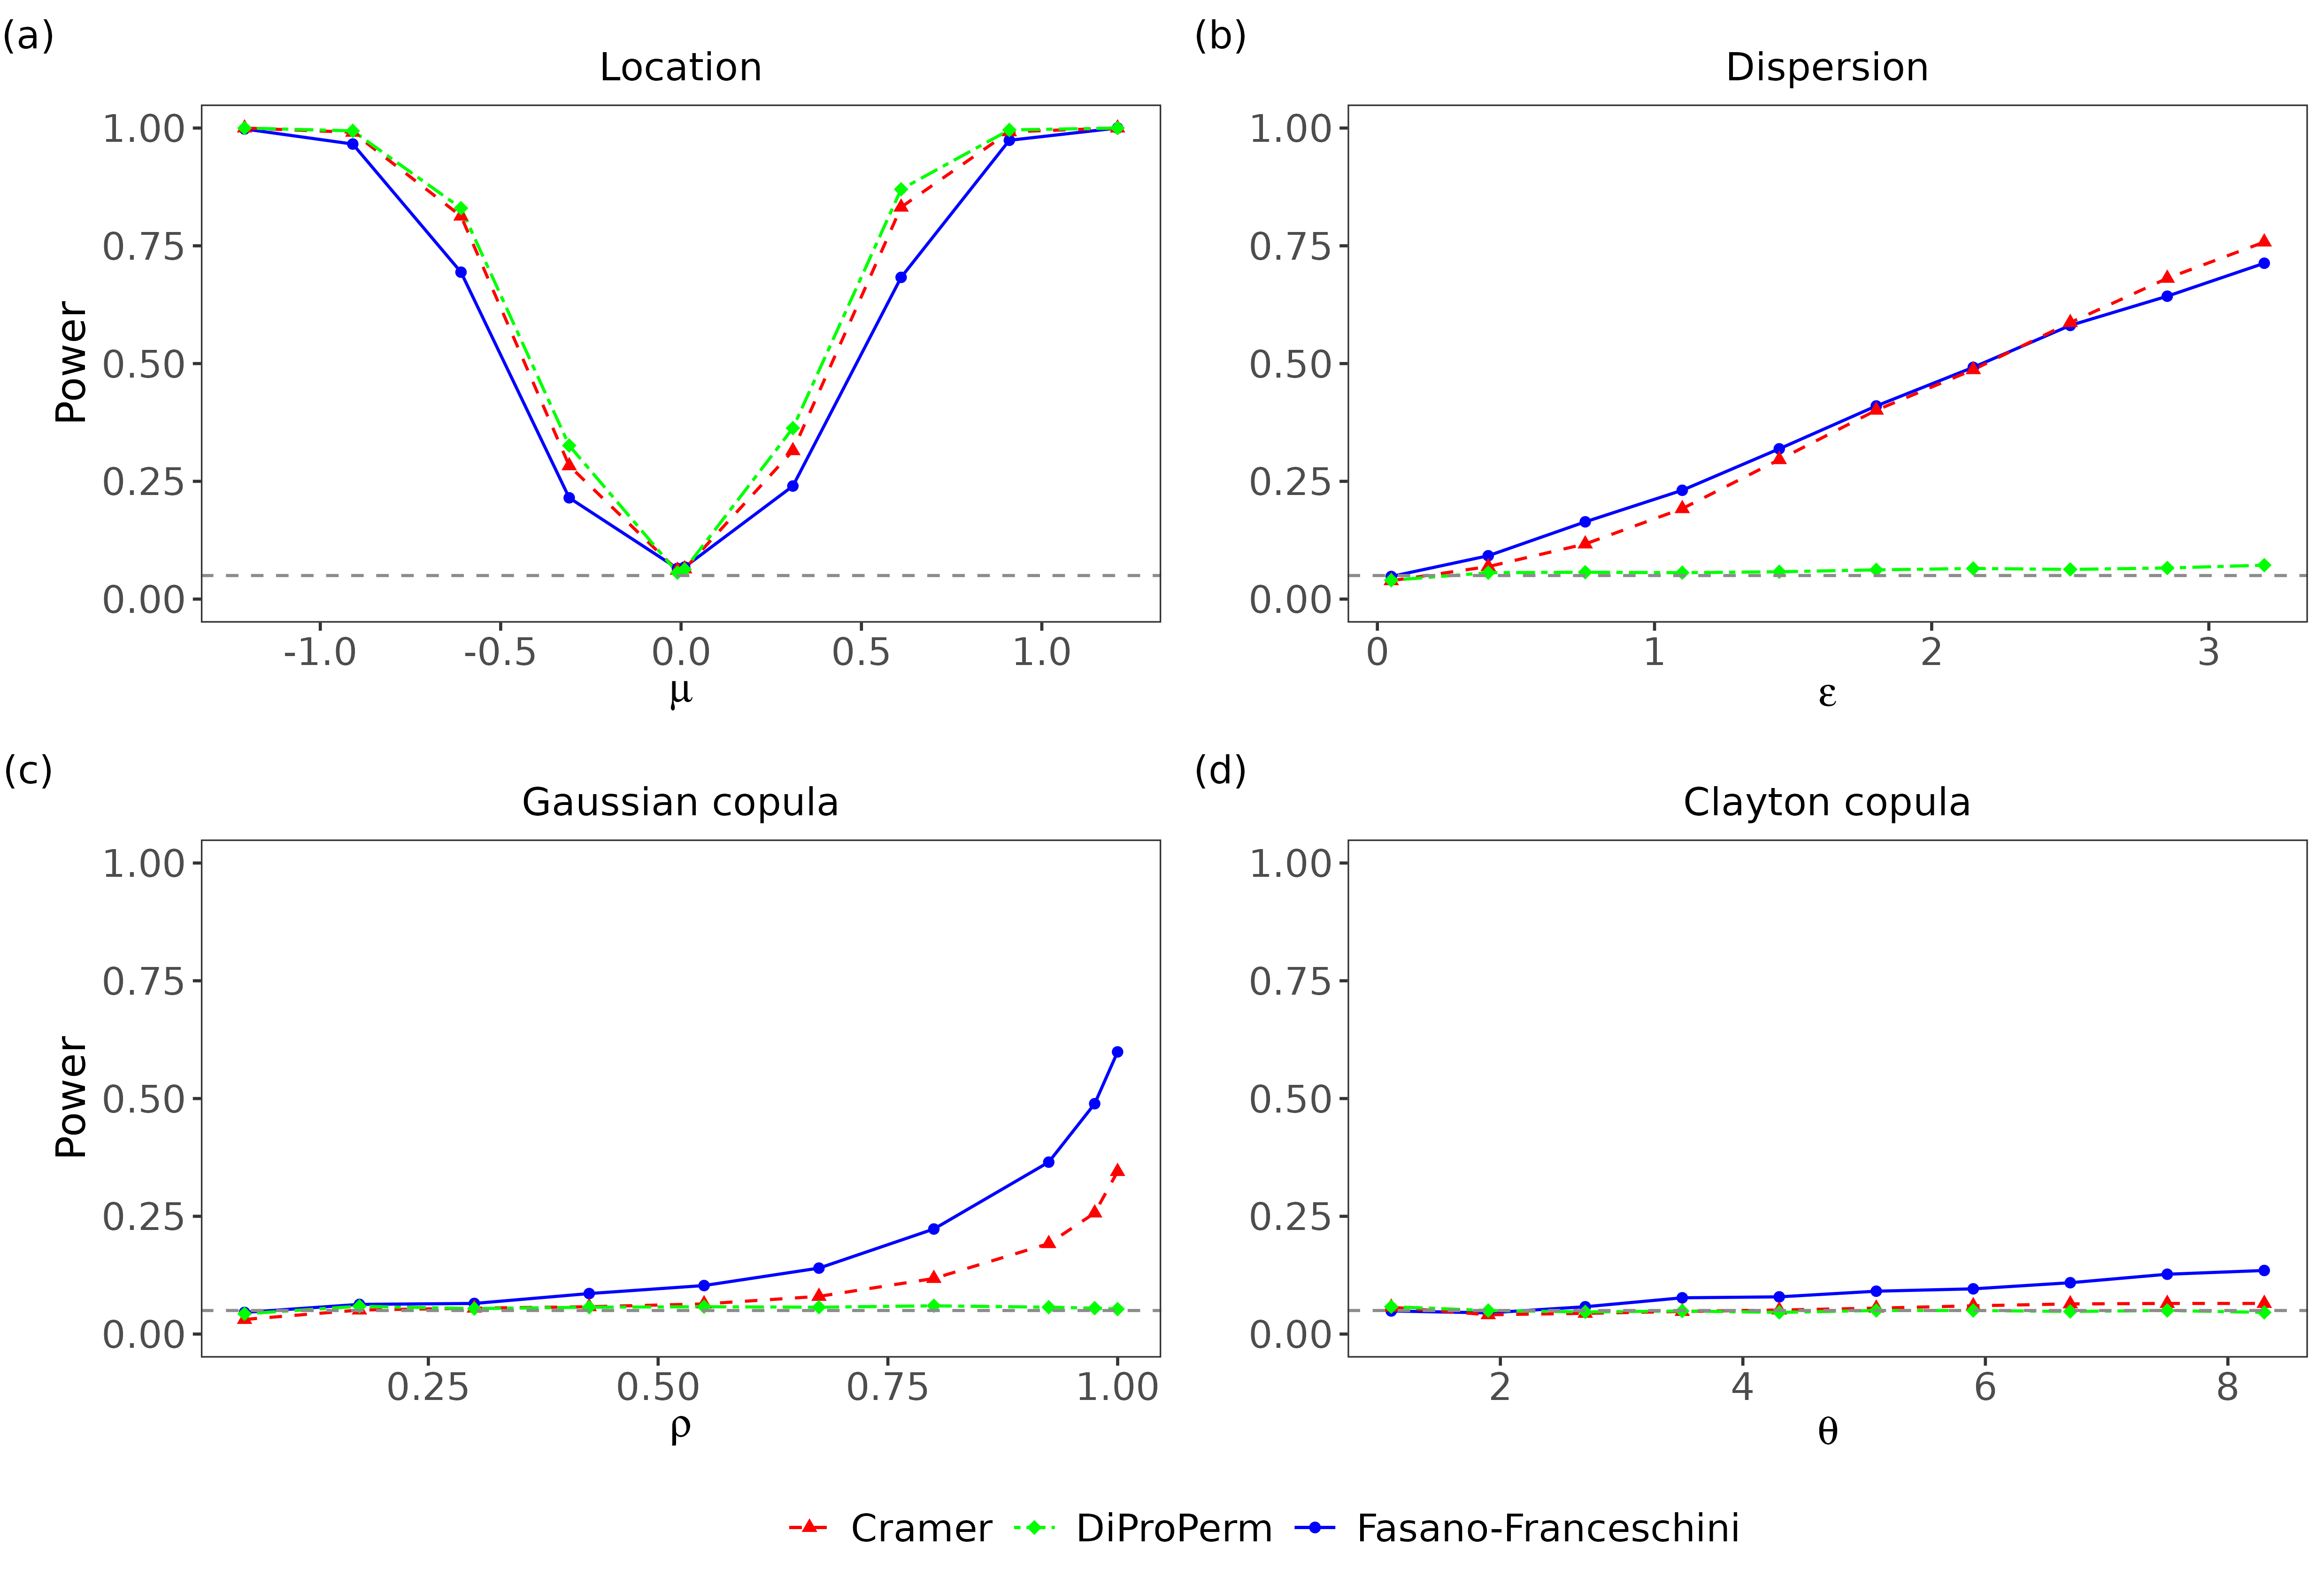
\includegraphics[scale=0.50]{figures/fig5.png}
\caption{Comparison of power of the Fasano--Franceschini, Cram\'er, and DiProPerm tests on various bivariate alternatives. (a) Location alternatives, with $S_{1}\sim N_{2}(\mathbf{0},\mathbf{I}_{2})$ and $S_{2}\sim N_{2}(\boldsymbol\mu,\mathbf{I}_{2})$. (b) Dispersion alternatives, with $S_{1}\sim N_{2}(\mathbf{0},\mathbf{I}_{2})$ and $S_{2}\sim N_{2}(\mathbf{0},\mathbf{I}_{2}+\varepsilon)$. (c) Gaussian copula alternatives, with $S_{1}\sim G_{2}(0)$ and $S_{2}\sim G_{2}(\rho)$. (d) Clayton copula alternatives, with $S_{1}\sim C_{2}(1)$ and $S_{2}\sim C_{2}(\theta)$.}
\label{figure:bivariate_power}
\end{figure}

We first examined the power of the tests on various bivariate alternatives (Figure~\ref{figure:bivariate_power}). All three tests had similar power across location alternatives, although the Cram\'er and DiProPerm tests did outperform the Fasano--Franceschini test. Across dispersion alternatives, the Cram\'er and Fasano--Franceschini tests had very similar powers. On Gaussian copula alternatives, the Fasano--Franceschini test had a consistently higher power than the Cram\'er test. This was also the case with Clayton copula alternatives, although none of the tests were able to achieve high power. The DiProPerm test was unable to achieve a power above the significance level of $\alpha=0.05$ on any of the dispersion or copula alternatives. This is likely due to the fact that in these instances, there is significant overlap between the high density regions of the two sampling distributions, making it difficult to find a separating hyperplane between samples drawn from them.

\begin{figure}[htbp]
\centering
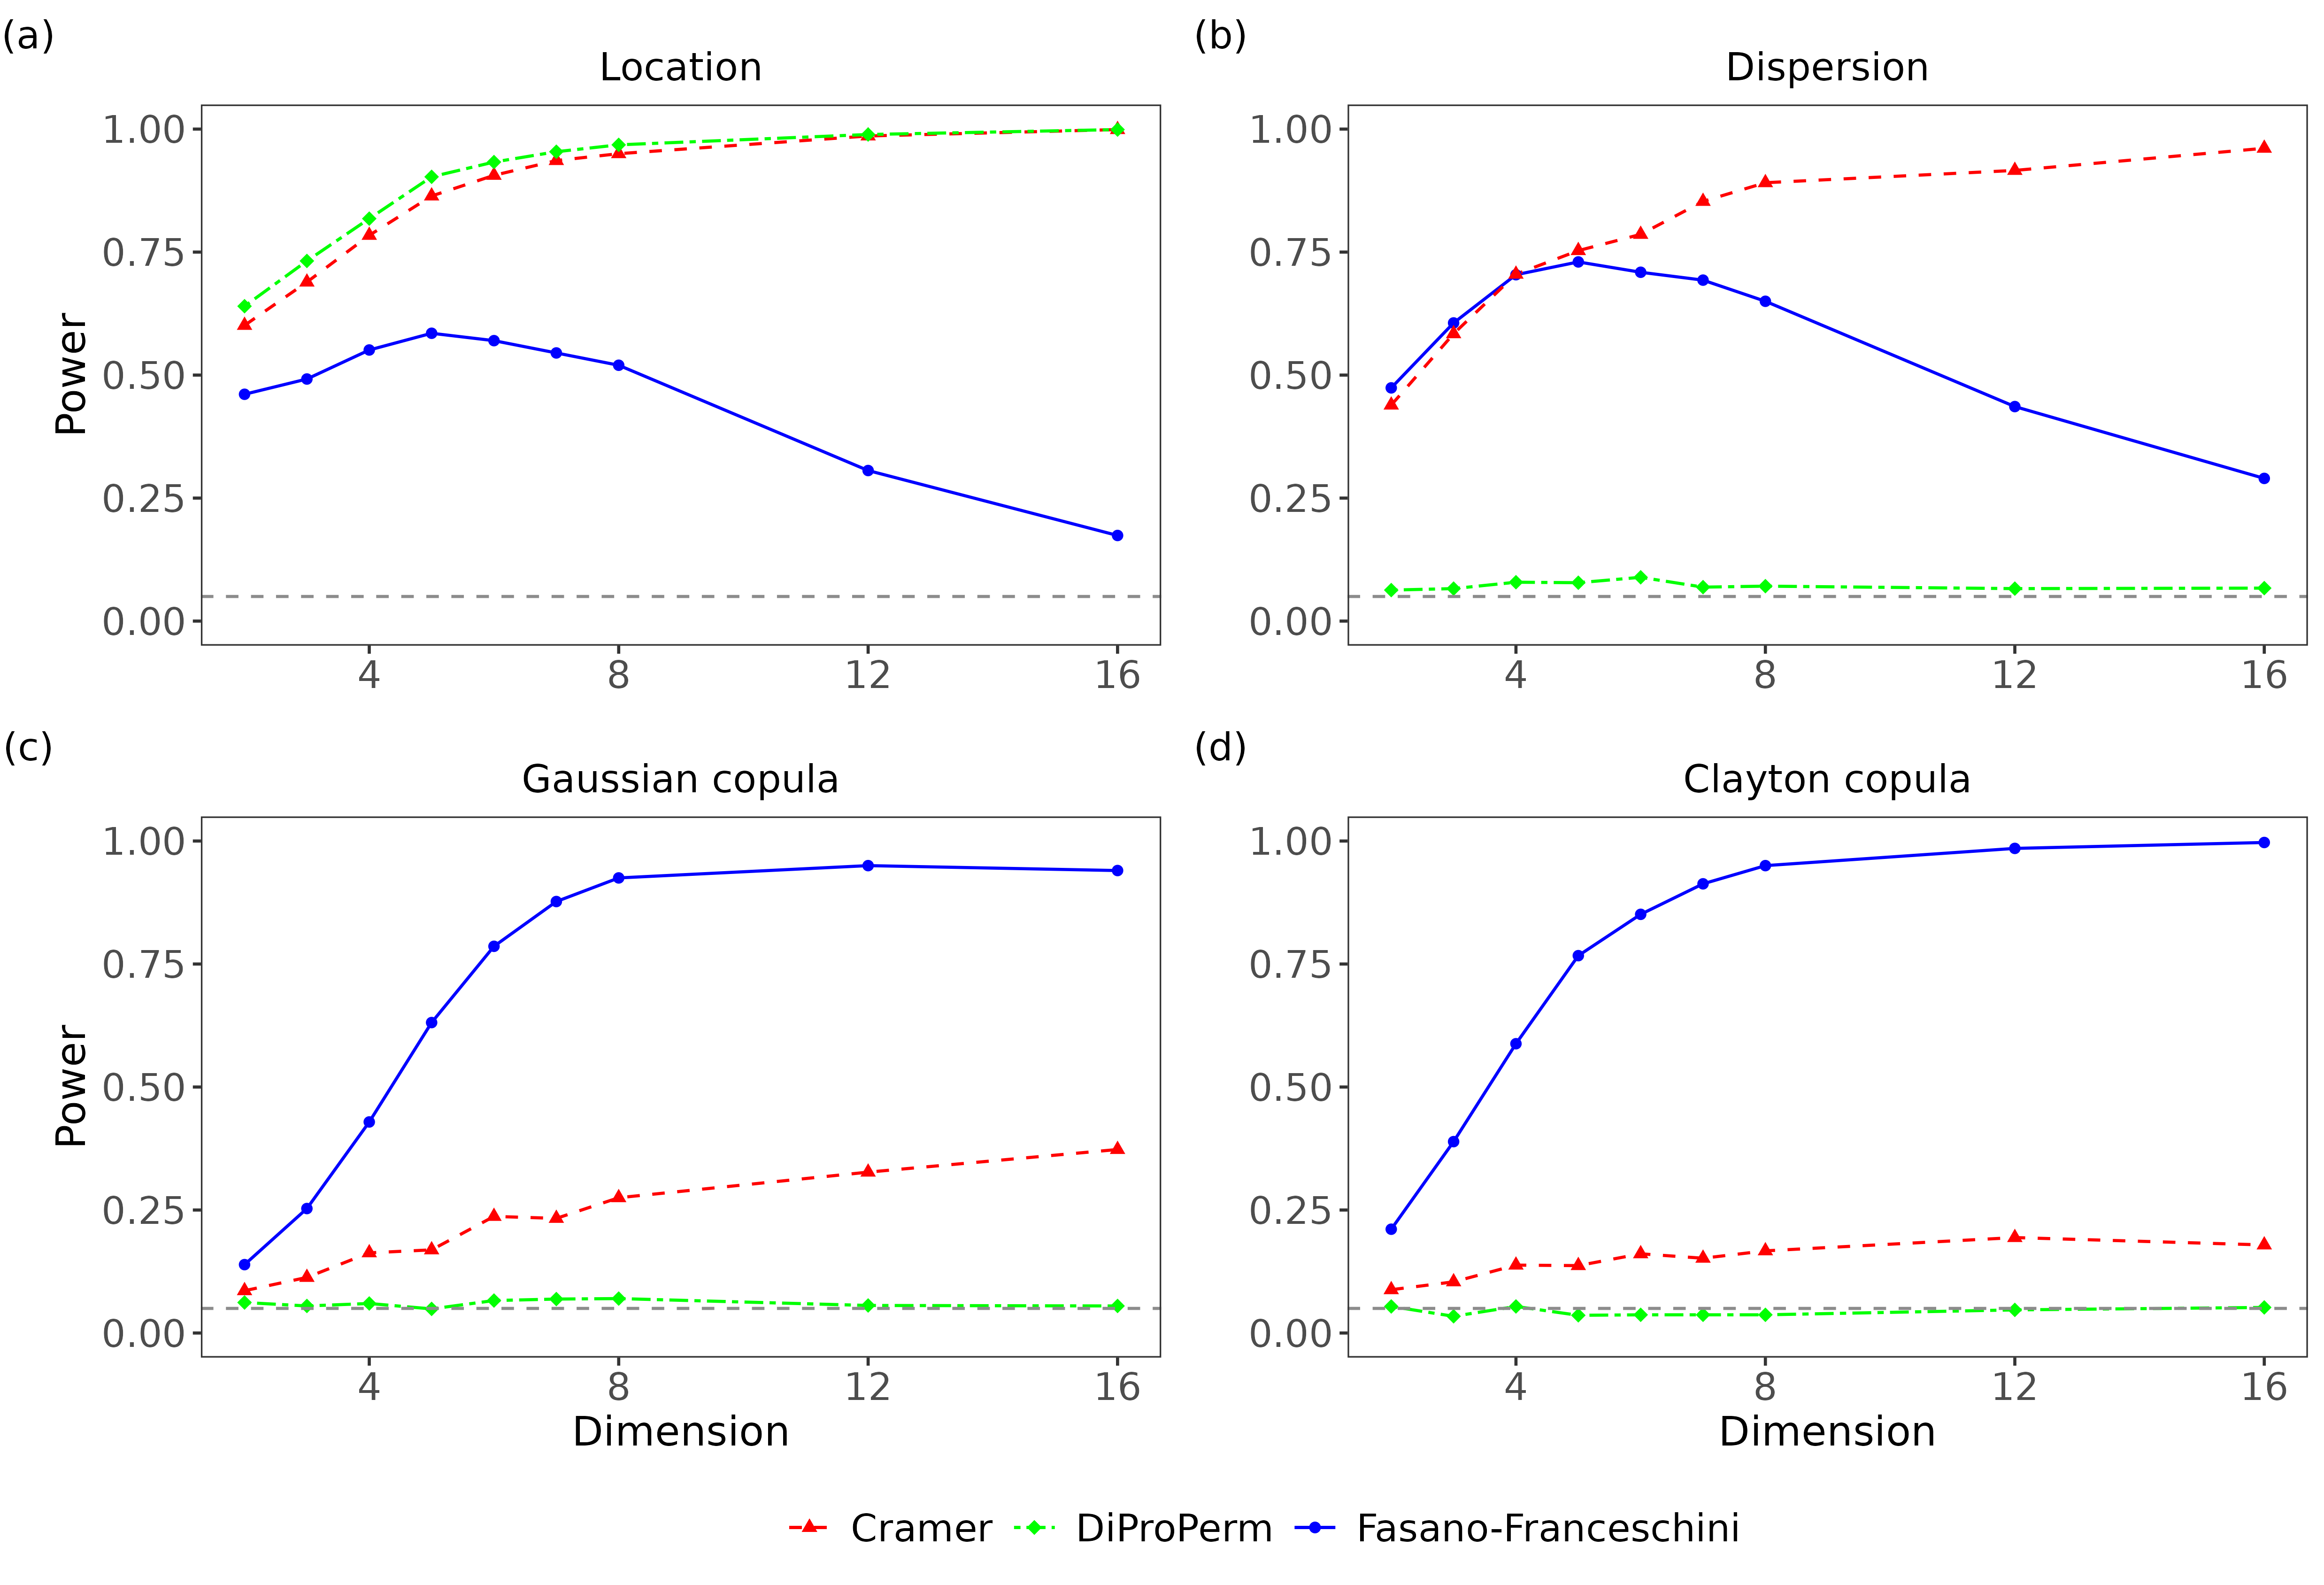
\includegraphics[scale=0.50]{figures/fig6.png}
\caption{Comparison of power of the Fasano--Franceschini, Cram\'er, and DiProPerm tests on fixed alternatives as the dimension of the data increases. (a) Location alternative, with $S_{1}\sim N_{d}(\mathbf{0},\mathbf{I}_{d})$ and $S_{2}\sim N_{d}(\mathbf{0.4},\mathbf{I}_{d})$. (b) Dispersion alternative, with $S_{1}\sim N_{d}(\mathbf{0},\mathbf{I}_{d})$ and $S_{2}\sim N_{d}(\mathbf{0},\mathbf{I}_{d}+1.5)$. (c) Gaussian copula alternative, with $S_{1}\sim G_{d}(0)$ and $S_{2}\sim G_{d}(0.6)$. (d) Clayton copula alternative, with $S_{1}\sim C_{d}(1)$ and $S_{2}\sim C_{d}(8)$.}
\label{figure:dimension_power}
\end{figure}

We next examined how the power of the three tests varied when the two sampling distributions were kept fixed but the dimension of the data increased (Figure~\ref{figure:dimension_power}). On the location alternative, the Cram\'er and DiProPerm tests again outperformed the Fasano--Franceschini test. In particular, for $d>5$, the Fasano--Franceschini steadily lost power as the dimension increased whereas the other tests gained power. On the dispersion alternative, the Cram\'er and Fasano--Franceschini tests had nearly identical powers through to $d=5$, but for higher dimensions the Cram\'er test consistently outperformed the Fasano--Franceschini test. On the other hand, for both the Gaussian and Clayton copula alternatives the Fasano--Franceschini test had a much higher power than the Cram\'er test. The DiProPerm test was still unable to attain a power above the significance level on the dispersion alternatives or either of the copula alternatives.

Overall, the Cram\'er and DiProPerm tests performed better than the Fasano--Franceschini test on location alternatives, especially as dimension increased. On dispersion alternatives, the Fasano--Franceschini and Cram\'er tests had comparable performance for low dimensions, but the Cram\'er test maintained a higher power for high dimensions. However, in these cases the marginal distributions differ, and thus a multivariate test is not strictly necessary as univariate tests could be applied to the marginals independently (with a multiple testing correction) to detect differences between the multivariate distributions. On copula alternatives, where a multivariate test is necessary, the Fasano--Franceschini test consistently outperformed both the Cram\'er and DiProPerm tests. Thus while the Fasano--Franceschini did not achieve the highest power in every case, we believe it to be the best choice as a general purpose multivariate two-sample goodness-of-fit test.

%%%%%%%%%%%%%%%%%%%%%%%%%%%%%%%%%%%%%%%%%%%%%%%%%%%%%%%%%%%%

\section{Summary}
This paper introduces the \pkg{fasano.franceschini.test} package, an R implementation of the multivariate two-sample goodness-of-fit test described by \citet{ff1987}. We provide users with a computationally efficient test that is applicable to data of any dimension and of any type (continuous, discrete, or mixed), and that demonstrates competitive performance with similar R packages. Complete package documentation and source code are available via the Comprehensive R Archive Network (CRAN) at \url{https://cran.r-project.org/web/packages/fasano.franceschini.test} and the package website at \url{https://braunlab-nu.github.io/fasano.franceschini.test}.

%%%%%%%%%%%%%%%%%%%%%%%%%%%%%%%%%%%%%%%%%%%%%%%%%%%%%%%%%%%%

\section{Computational details}
The results in this paper were obtained using R 4.2.0 with the packages \pkg{fasano.franceschini.test} 2.2.1, \pkg{diproperm} 0.2.0, \pkg{cramer} 0.9-3, \pkg{MASS} 7.3-60, \pkg{copula} 1.1-2, and \CRANpkg{microbenchmark} 1.4.10 \citep{microbenchmarkR}. Plots were generated using \CRANpkg{ggplot2} 3.4.2 \citep{ggplotR} and \CRANpkg{patchwork} 1.1.1 \citep{patchworkR}. All computations were done using the Quest high performance computing facility at Northwestern University.

%%%%%%%%%%%%%%%%%%%%%%%%%%%%%%%%%%%%%%%%%%%%%%%%%%%%%%%%%%%%

\section{Acknowledgments}
This research was supported in part through the computational resources and staff contributions provided for the Quest high performance computing facility at Northwestern University which is jointly supported by the Office of the Provost, the Office for Research, and Northwestern University Information Technology. 
%
Funding for this work was provided by NIH/NIA R01AG068579, Simons Foundation 597491-RWC01, and NSF 1764421-01.

%%%%%%%%%%%%%%%%%%%%%%%%%%%%%%%%%%%%%%%%%%%%%%%%%%%%%%%%%%%%

\bibliography{puritz-nesscohn-braun}

%%%%%%%%%%%%%%%%%%%%%%%%%%%%%%%%%%%%%%%%%%%%%%%%%%%%%%%%%%%%

\address{Connor Puritz\\
  Department of Engineering Sciences and Applied Mathematics, Northwestern University\\
  Evanston, IL 60208\\
  ORCiD: 0000-0001-7602-0444\\
  Email: \email{connorpuritz2025@u.northwestern.edu}}

\address{Elan Ness-Cohn\\
  Department of Molecular Biosciences, Northwestern University\\
  Evanston, IL 60208\\
  ORCiD: 0000-0002-3935-6667\\
  Email: \email{elan.ness-cohn@northwestern.edu}\\
  Website: \url{https://sites.northwestern.edu/elannesscohn/}}

\address{Rosemary Braun\\
  Department of Molecular Biosciences, Northwestern University\\
  Evanston, IL 60208\\
  ORCiD: 0000-0001-9668-9866\\
  Email: \email{rbraun@northwestern.edu}\\
  Website: \url{https://sites.northwestern.edu/braunlab/}}
  